\chapter{Di-$b$-jet Search: Outline and Event Selection}
\label{sec:evt}

In Chapter~\ref{sec:theo} it was shown that many Beyond Standard Model theories
predict new particles decaying to one or two $b$-quarks that could be produced by the LHC.
Chapters~\ref{sec:det},~\ref{sec:obj}~and~\ref{sec:trig}
described the detectors and reconstruction techniques used to observe such an event in the ATLAS detector.
Hence, I have now outlined the motivation and the tools required to perform
a search for resonances decaying to one or two $b$-jets,
an analysis that is called a di-$b$-jet search.

In Chapters~\ref{sec:evt},~\ref{sec:bkg}~and~\ref{sec:lim}
I will describe the di-$b$-jet search analysis using the ATLAS detector.
Each chapter will describe a separate part of the analysis,
as described in Section~\ref{sec:evt-outline}.
Three related di-$b$-jet analyses are described in
the following chapters
each using a different data-set.
The data-sets are described in Section~\ref{sec:evt-datasets}
and each analysis will be clearly referenced in any discussion.

\section{Analysis Outline}
\label{sec:evt-outline}

The strategy used for the di-$b$-jet analysis
can be split up into broadly three parts.
A brief outline of the parts is given here,
and full detail can be fround in the relevant chapter.

\begin{itemize}[leftmargin=*]
\item\textbf{Di-$b$-jet Event Selection:} (\textit{Chapter~\ref{sec:evt}})\\
  The first step is to select events that are consistent with a resonance decaying to one or two $b$-quarks.
  Briefly, we will require two high-momentum jets and consider two $b$-tag categories;
  one where both jets have been $b$-tagged or where at least one jet has been $b$-tagged.
  The remainder of the chapter will focus on details of analysis selection;
  Section~\ref{sec:evt-datasets} will describe the data-sets used,
  Section~\ref{sec:evt-s+b} will describe the signal and backgrounds
  considered when defining the selections
  and Section~\ref{sec:evt-sel} will set out
  the details of the event selection used for each of the data-sets.
  \\
\item\textbf{Search Phase:} (\textit{Chapter~\ref{sec:bkg}})\\
  Once events have been selected the next part of the analysis aims to determine if there is
  is a new particle in the selected events; this step is known as the `search phase'.
  For this we will use the $m_{jj}$ spectrum, where $m_{jj}$ is the invariant mass of the two leading jets.
  A new particle will appear as a resonance (or `bump') on the smoothy falling
  $m_{jj}$ distibution from QCD multi-jet, as illustrated in Figure~\ref{fig:evt-dijet_schem}.
  A fit function is used to model the smoothly falling QCD background and a
  a model-independant search for for resonances is performed using the BumpHunter algorithm.
  Chapter~\ref{sec:bkg} contains a full description of the search phase strategy.
  %including tests of the fitting functions used and the results of the search phase in the data-sets considered.
  \\
  
  \begin{figure}[!hbt]
  \begin{center}
    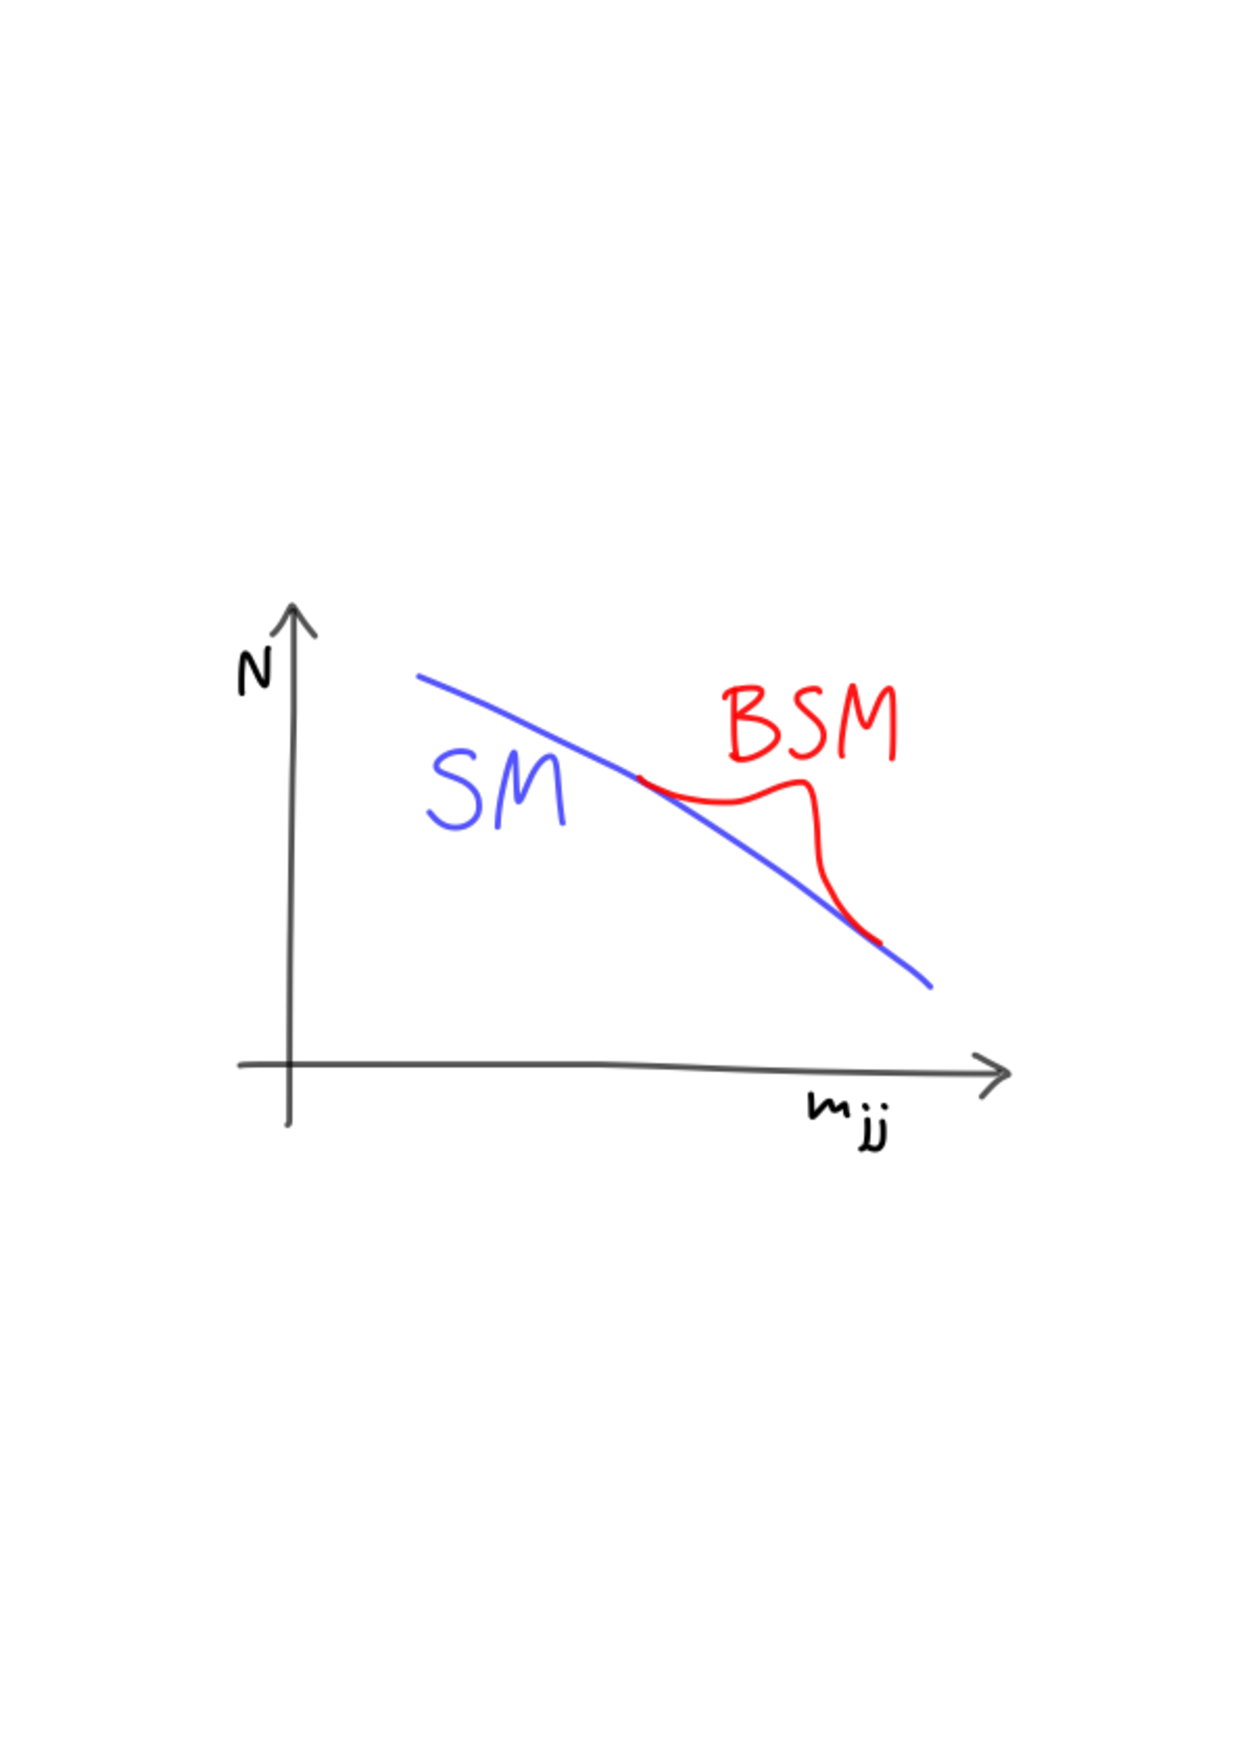
\includegraphics[width=0.5\linewidth, angle=0]{figs/Dibjet/Gen/dijet_schem.pdf}
  \end{center}
  \caption[A cartoon illustrating the use of dijet invariant mass ($m_{jj}$) distribution in the search phase of the di-$b$-jet analysis.
    Shown is the expected smoothly falling  distribution of multijet QCD (labelled as SM)
    and a resonance shape due to Beyond Standard Model particle (labelled as BSM)]
          {A cartoon illustrating the use of the dijet invariant mass ($m_{jj}$) distribution in the search phase of the di-$b$-jet analysis.
            Shown is the smoothly falling distribution from multijet QCD (SM)
            and a resonance shape caused by a Beyond Standard Model particle (BSM)~\textit{Reference Lene}.}
          \label{fig:evt-dijet_schem}
  \end{figure}
 
\item\textbf{Limit Setting:} (\textit{Chapter~\ref{sec:lim}})\\
  If, in the search phase stage of the analysis, no significant evidence of signal is
  found then it is desirible to quantify what cross-sections can be excluded as a result.
  95\% confidence lower mass limits are set on the two benchmark signals considered
  (described in Section~\ref{sec:evt-s+b}.
  The limit-setting methodology, description of systematics considered
  and final limit results in the data sets considered is contained in Chapter~\ref{sec:lim}.

\end{itemize}




\section{Datasets}
\label{sec:evt-datasets}

\section{Signal and Backgrounds}
\label{sec:evt-s+b}

\section{Event Selection}
\label{sec:evt-sel}

\subsection{Jet Selection}
\label{sec:evt-sel-jet}

\subsection{Event Kinematics}
\label{sec:evt-sel-event}

\subsection{$b$-Tagging}
\label{sec:evt-sel-btag}

\subsection{Acceptance}
\label{sec:evt-sel-acc}
